\vspace{10pt}

{\centering\subsection*{何宇州:沙哈拉沙漠探险之旅}}

\addcontentsline{toc}{subsection}{何宇州:沙哈拉沙漠探险之旅}

\renewcommand{\leftmark}{何宇州:沙哈拉沙漠探险之旅}

\begin{figure}[htbp]

\centering

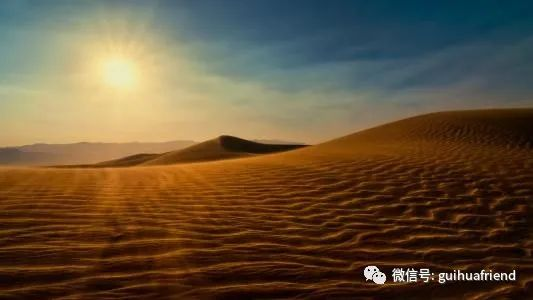
\includegraphics[width = .5\textwidth]{./ch/5.jpg}

\end{figure}



毕业后,我和胆大包天的表哥、探险大师—明刚准备去其面积就大于美国国土的撒哈拉沙漠探险。

我们在探险的前一天准备了很多物品。我们知道在沙漠中最缺的就是水,所以我们就把一个背包里装满了水。我们还带了药品,因为撒哈拉沙漠中有许多危险的动物。我们把东西都准备好后就去找明刚了。找到了明刚,他对我们说道:“今天我们好好休息一下,明天我们再去。”

第二天,我们去了撒哈拉沙漠,我们本来十分开心,可突然一位本地老人严肃地对我们说:“你们要去撒哈拉沙漠吗?如果你们要去的话可要小心了,那里有十分多的毒物,那里的蜈蚣至少有60厘米长,还有毒蚺、蟒蛇、响尾蛇等!”我们听了老人的话后十分惊讶。心想:原来撒哈拉沙漠这么危险啊!可明刚却冷静地说道:“谢谢您,我们知道了!”

我们去撒哈拉沙漠中的前几天还没有什么事。可是今天我们看到了人骨,我们吓得胆战心惊。我们离开了那个地方后,我的表哥一不小心踩到了一只毒蜈蚣,明刚连忙把一个东西向毒蜈蚣那里一扔,毒蜈蚣一下就没气了。明刚让我们把鼻子捂住,那毒蜈蚣的身体中发出了一种黑绿色的气体。明刚看气体消失后对我们说道:“我扔出去的是二氧毒气弹,闻到的话会立刻死亡的!”

我们在这件事过后就十分小心了,因为表哥差点就被蜈蚣咬到了,之后我们还经历了流沙、毒蝎......最后我们历经千辛万苦终于回到了家。

这就是我惊险刺激的沙哈拉沙漠之旅,也让我学到不少的求生技巧。





\vspace{10pt}



作者:五(3)班 何宇州



指导老师:刘婷



投稿:2021年6月10日



发表:2021年6月11日






                



\vspace{10pt}

\hline



